%\documentclass[10pt,a4paper]{article}
\documentclass[12pt,a4paper]{article}

\usepackage[utf8]{inputenc}
\usepackage{hyperref}
\usepackage{polski}
\usepackage{graphicx}
\usepackage{listings}
\usepackage{algorithm}
\usepackage{algorithmic}

\usepackage{hyperref}
%\usepackage{antpolt}
\usepackage{amssymb}
\usepackage{multicol}
\usepackage{fancyvrb}

\usepackage{color}

%\setlength{\topskip}{0mm} \setlength{\footskip}{0mm} \setlength{\topmargin}{0mm} \setlength{\marginparwidth}{0mm}
%\setlength{\headsep}{2mm} \setlength{\headheight}{0mm} \setlength{\textheight}{250mm}
%\setlength{\textwidth}{160mm} \setlength{\oddsidemargin}{0mm} \setlength{\evensidemargin}{0mm}

\setlength{\topskip}{0mm} \setlength{\topmargin}{0mm}
\setlength{\oddsidemargin}{0mm} \setlength{\evensidemargin}{0mm}
\setlength{\marginparwidth}{0mm} \setlength{\headsep}{0mm}
\setlength{\headheight}{0mm} \setlength{\textheight}{240mm}
\setlength{\textwidth}{170mm}


\floatname{algorithm}{Algorytm}
\renewcommand{\lstlistlistingname}{Spis listingów}
\renewcommand{\lstlistingname}{Listing}


% \k{a} \'c \k{e} \l{} \'n \'o \'s
% \'z \.z \k{A} \'C \k{E} \L{} \'N
% \'O \'S \'Z \.Z 

\lstset{literate=
  {á}{{\'a}}1 {é}{{\'e}}1 {í}{{\'i}}1 {ó}{{\'o}}1 {ú}{{\'u}}1
  {Á}{{\'A}}1 {É}{{\'E}}1 {Í}{{\'I}}1 {Ó}{{\'O}}1 {Ú}{{\'U}}1
  {à}{{\`a}}1 {è}{{\`e}}1 {ì}{{\`i}}1 {ò}{{\`o}}1 {ù}{{\`u}}1
  {À}{{\`A}}1 {È}{{\'E}}1 {Ì}{{\`I}}1 {Ò}{{\`O}}1 {Ù}{{\`U}}1
  {ä}{{\"a}}1 {ë}{{\"e}}1 {ï}{{\"i}}1 {ö}{{\"o}}1 {ü}{{\"u}}1
  {Ä}{{\"A}}1 {Ë}{{\"E}}1 {Ï}{{\"I}}1 {Ö}{{\"O}}1 {Ü}{{\"U}}1
  {â}{{\^a}}1 {ê}{{\^e}}1 {î}{{\^i}}1 {ô}{{\^o}}1 {û}{{\^u}}1
  {Â}{{\^A}}1 {Ê}{{\^E}}1 {Î}{{\^I}}1 {Ô}{{\^O}}1 {Û}{{\^U}}1
  {Ã}{{\~A}}1 {ã}{{\~a}}1 {Õ}{{\~O}}1 {õ}{{\~o}}1
  {œ}{{\oe}}1 {Œ}{{\OE}}1 {æ}{{\ae}}1 {Æ}{{\AE}}1 {ß}{{\ss}}1
  {ű}{{\H{u}}}1 {Ű}{{\H{U}}}1 {ő}{{\H{o}}}1 {Ő}{{\H{O}}}1
  {ç}{{\c c}}1 {Ç}{{\c C}}1 {ø}{{\o}}1 {å}{{\r a}}1 {Å}{{\r A}}1
  {€}{{\euro}}1 {£}{{\pounds}}1 {«}{{\guillemotleft}}1
  {»}{{\guillemotright}}1 {ñ}{{\~n}}1 {Ñ}{{\~N}}1 {¿}{{?`}}1
  {ł}{\l{}}1 {ś}{{\'s}}1 {ź}{{\.z}}1  {ó}{{\'o}}1
}

\begin{document}
\pagestyle{empty}

%
%  strona tytułowa
%

\begin{center}
\textsc{\Huge{Uniwersytet Zielonogórski}}\\
\LARGE{Wydział Informatyki, Elektrotechniki i Automatyki}\\
\vspace{0.5cm}
\Large{Platforma .NET -- Projekt}\\
Prowadzący: dr inż. Marek Sawerwain\\ \vspace{1cm}
\LARGE{Tytuł raportu/sprawozdania}\\
\vspace{0.5cm} 
\Large{Wykonał: Damian Radecki, Grupa dziekańska: 33-INF-SSI-SP} \\
\Large{Projekt realizowano razem z: \\ Damian Kurkiewicz}\\
\Large{Data oddanie projektu: DD mmmm YYYY}
\vspace{1cm}
\begin{flushleft}
	Ocena: ..........................................
\end{flushleft}
\vspace{1cm}
\end{center}



%
% spis treści
%

\begin{multicols}{2}
	\footnotesize
	\tableofcontents
\end{multicols}


%
% spis listingów
%

\begin{multicols}{2}
	\footnotesize
	\lstlistoflistings
\end{multicols}




\noindent\makebox[\linewidth]{\rule{0.6\paperwidth}{0.4pt}}

\begin{flushleft}
	\emph{Motto:}\\
	\textit{Pisanie raportu przywilejem każdego studenta.}
\end{flushleft}

% 1. Wprowadzenie
% 2. Użyte technologie
% 3. Projekt i implementacji
% 4. Testy (jednostkowe, testy UI)
% 5. Wdrożenie -- instalacja
% 6. Wkład poszczególnych Autorek/Autorów projektu
% 7. Podsumowanie


\section{Wprowadzenie} 

\subsection{Aplikacje czasu rzeczywistego}
\hspace*{0.7cm} Aplikacje działające na żywo oferują wiele korzyści, które są sporym ułatwieniem dla użytkowników podczas używania takiej aplikacji. Czynności wykonywane
bez odświeżania strony nie tylko skracają czas wykonywania czynności czy obsługiwania samej witryny to jeszcze znacznie ułatwiają komunikację, unikają 
blokowania strony i tworzą bardziej intuicyjny interface. Takie aplikacje internetowe staja się normą w dzisiejszych czasach. Każde przeładowanie strony jest
nie komfortowe i stwarza pewnego rodzaju niebezpieczeństwo wykradnięcia danych. Serwisy internetowe obsługujące komunikację real-time z klientem są lepiej 
zabezpieczone i działają wydajnościowo lepiej. Powstawało wiele technologii do wsparcia komunikacji na żywo, które działają zarówno po stronie witryny i
serwera. Są to między innymi WebSocket, SignalR, RabbitMQ czy Apache Kafka. Wszystkie z nich są dziś globalnie używane do wsparcia przekazu informacji.

\subsection{Opis działania}
\hspace*{0.7cm} Projekt chatu na żywo jest aplikacją, która wspiera komunikację między użytkownikami, aby ich konwersacje nie działały w stylu w jakim działa klasyczny serwer
e-mail. Założenie projektu są takie, aby użytkownicy bez przeładowania strony mogli wymieniać miedzy sobą wiadomości. Dodatkowo wszelkie powiadomienia
przychodzą również bez zbędnego odświeżania witryny. Sprawia to, że witryna jest bardziej intuicyjna, łatwiejsza i szybsza w obsłudze. Taka architektura
aplikacji jest przyjazna użytkownikowi, od którego będzie wymagana minimalny wysiłek w trakcie używania strony. Celem takiej aplikacji jest też maksymalne 
bezpieczeństwo wspierane przez bearen token i autoryzację użytkowników z zachowaniem szyfrowania danych poufnych. Architektura zapewnia, że nie będziemy otrzymywać wiadomości od niezaakceptowanych użytkowników lecz daje możliwość uczestnictwa w czatach posiadających osoby nieznajome poprzez mechanizm grup. W grupach każdy użytkownik może zaprosić swoich znajomych co może spowodować komunikację między nieznajomymi w danym czacie.


\subsection{Grupa docelowa}
\hspace*{0.7cm} Grupą docelową są wszyscy użytkownicy którzy cenią sobie bezpieczeństwo i wygodę. Chcą szybko skomunikować się ze swoimi przyjaciółmi bądź grupą docelową
bez żadnych opóźnień czy niepotrzebnych przeładować strony. Są pewni tego, że ich dane są przechowywane w bezpiecznym miejscu i nikt nie wkradnie się na ich
konto. Mogą to być zarówno firmy, które chcą komunikować się między sobą i ewentualnie z klientami poprzez utworzenie chatu dla grupy użytkowników jak i dla szkół, uniwersytetów, grup pracowników, przyjaciół czy kolegów. 


\section{Użyte technologie}

\subsection{.Net Core} 			%razem
\hspace*{0.7cm} Popularny, nowoczesny i wydajny framework oparty o otwartoźródłowa implementację, który został wydany w 2016 roku do ogólnego przeznaczenia. Stanowi zestaw bibliotek pozwalający tworzyć wieloplatformowe aplikacje o wysokim stopniu bezpieczeństwa. Framework ten pozwala na pisanie aplikacji między innymi przeznaczonych do obliczeń chmurowych, IoT oraz jak w naszym przypadku do pisania web serwisu. 

\begin{figure}[h]
	\centering
	
\includegraphics[width=0.3\linewidth]{dotnet5_platform}
	\caption{Logo .Net Core}
	\label{fig:dotnet5platform}
\end{figure}

Framework .Net Core został przez nas wybrany, ponieważ jest to nowa oraz dobrze prosperująca technologia wprowadzająca dużą dawkę świeżości podczas tworzenia nowego oprogramowania. Posiada wsparcie dla tworzenia web serwisów opartych o metodykę REST, poprzez dodanie nowych i gotowych do działania bibliotek. Platforma .Net Core jest znacznie wydajniejsza od .Net Framework. Wprowadza znaczące usprawnienia przekładające się na szybkość działania pisanych programów. Architektura przedstawia się w sposób następujący.\newline

\begin{figure}[h]
	\centering
	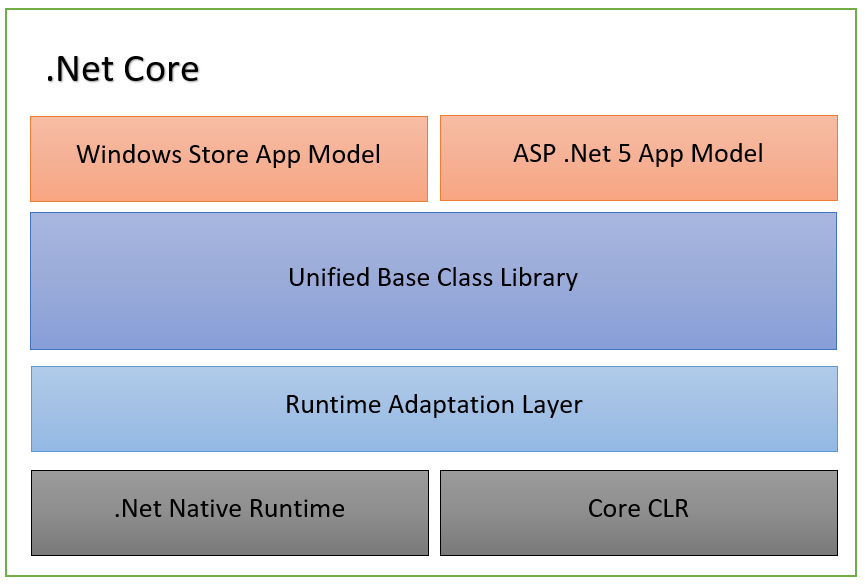
\includegraphics[width=0.7\linewidth]{net-Core-1}
	\caption{Architektura .NET Core}
	\label{fig:net-core-1}
\end{figure}

\subsection{Entity Framework}   %ja

\hspace*{0.7cm} Entity Framework to zestaw technologii ADO.NET, obsługujące opracowywanie aplikacji zorientowanych na dane. Framework ten pozwala modelować konkretne jednostki, relację czy też logikę działania bazy danych. Obsługuję wiele systemów magazynowania danych takich jak na przykład MySQL, który to został przez nas wybrany do realizacji projektu. Całość jest konfigurowalna z poziomu kodu co jest bardzo wygodnym rozwiązaniem. Pozwala deweloperom na współpracę z danymi w postaci obiektów. Model fizyczny jest rafinowany przez administratorów bazy danych w celu zwiększenia wydajności, ale programiści piszący kod aplikacji przede wszystkim zawężają się do pracy z modelem logicznym, pisząc zapytania SQL i wywołując procedury składowane. Modele domen są zwykle używane jako narzędzie do przechwytywania i komunikowania się z wymaganiami aplikacji, często tak jak w przypadku diagramów obojętnych, które są wyświetlane i omówione w wczesnych etapach projektu, a następnie porzucone. Wiele zespołów programistycznych pomija Tworzenie modelu koncepcyjnego i rozpoczyna się od określenia tabel, kolumn i kluczy w relacyjnej bazie danych.\newline

\begin{figure}[h]
	\centering
	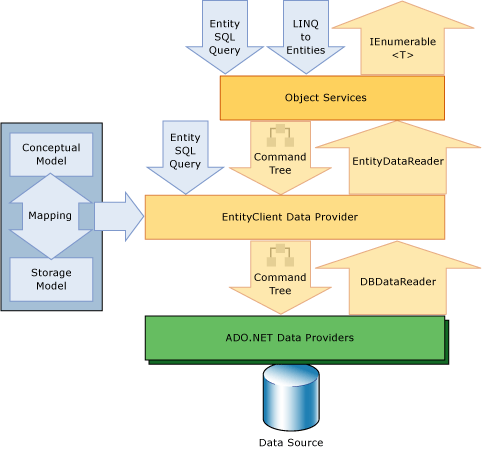
\includegraphics[width=0.7\linewidth]{entity}
	\caption{Architektura Entity Framework do uzyskania dostępu do danych}
	\label{fig:entity}
\end{figure}


\subsection{SignalR} 			%kurek

\hspace*{0.7cm} Biblioteka dla dewelpoarów ASP.NET, która przyśpiesza proces dodawania funkcji sieci web w czasie rzeczywistym do aplikacji. Często wykorzystuje się tą bibliotekę w czatach internetowych, lecz może ona o wiele więcej. SignalR może być używany też w takich aplikacjach jak pulpity nawigacyjne, aplikacje do monitorowania czy formularze działające w czasie rzeczywistym. Biblioteka umożliwia również zupełnie nowe typy aplikacji internetowych, które wymagają aktualizacji wysokiej częstotliwości z serwera, na przykład gier w czasie rzeczywistym.
Komunikacja między stroną a serwerem odbywa się poprzez tak zwane Hub'y. Bardzo dobrze ukazuje to rysunek poniżej. \newline

\begin{figure}[h]
	\centering
	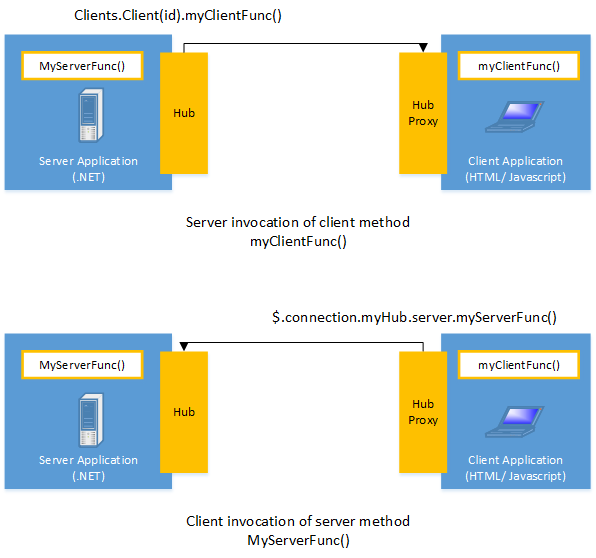
\includegraphics[width=0.7\linewidth]{signalr}
	\caption{SignalR przykład działania}
	\label{fig:signalr}
\end{figure}

\subsection{MySql} 				%ja

\hspace*{0.7cm} Baza danych rozwijana przez firmę Oracle. MySql jest to otwarto źródłowy system zarządzania relacyjnymi bazami danych. System ten obsługuję język zapytań SQL, który służy do pisania zapytań do tej bazy. MySql jest relacyjną bazą danych. Model relacyjny w prosty i intuicyjny sposób przedstawia dane w tabelach. Każdy wiersz w tabeli jest rekordem z unikatowym identyfikatorem zwanym kluczem. Kolumny tabeli zawierają atrybuty danych, a każdy rekord zawiera zwykle wartość dla każdego atrybutu, co ułatwia ustalenie relacji między poszczególnymi elementami danymi.\newline
 
\begin{figure}[h]
	\centering
	
\includegraphics[width=0.7\linewidth]{mysql-logo}
	\caption{Logo MySQL}
	\label{fig:mysql-logo}
\end{figure}

\newpage
\subsection{Angular} 			%kurek

\hspace*{0.7cm} Otwarto źródłowy framework JavaScript, zaprojektowany i napisany przez inżynierów z Google. Ich celem było zrewolucjonizowanie projektowania części wizualnej stron internetowych. Szybko zyskał popularność wśród programistów JavaScript, którzy zaczęli odstawiać go na rzecz jQuery. Jego największą zaletą oraz najbardziej rozpoznawalną cechą jest integracja z atrybutami HTML. Framework ten umożliwia proste wdrożenie wzorca MVC(Model-View-Controller), dzięki czemu testowanie jak i rozwój aplikacji nie sprawia wielu problemów.

\begin{figure}[h]
	\centering
	
\includegraphics[width=0.7\linewidth]{AngularJS_logo}
	\caption{Logo Angular}
	\label{fig:angularjslogo}
\end{figure}


\section{Projekt}

\subsection{Struktura projektu} %razem

Diagram pokązujący architekturę całego projektu opisuje główne komponenty i występujące między nimi połączenia. Strona internetowa napisana w Angularze jest podłączona bezpośrednio z signalR i web serwisem. Miedzy nim występują połączenia dwukierunkowe. Z tym pierwszym strona internetowa utrzymuje stałe połączenie, aby zapewnić natychmiastową wymianę danych. Drugi wymieniony komponent odpowiada na zadane żądania. SignalR został wbudowany w web serwis jako integralna część, ale jest traktowany osobno, ponieważ utrzymuje z klientem innego typu połączenie. Między nimi także następuje wymiana danych. Ostatnim komponentem projektu jest baza danych, która jest podłącza tylko do web serwisu. To on stanowi most do pobierania wszelkich zawartych tam informacji. 

\begin{figure}[h]
	\centering
	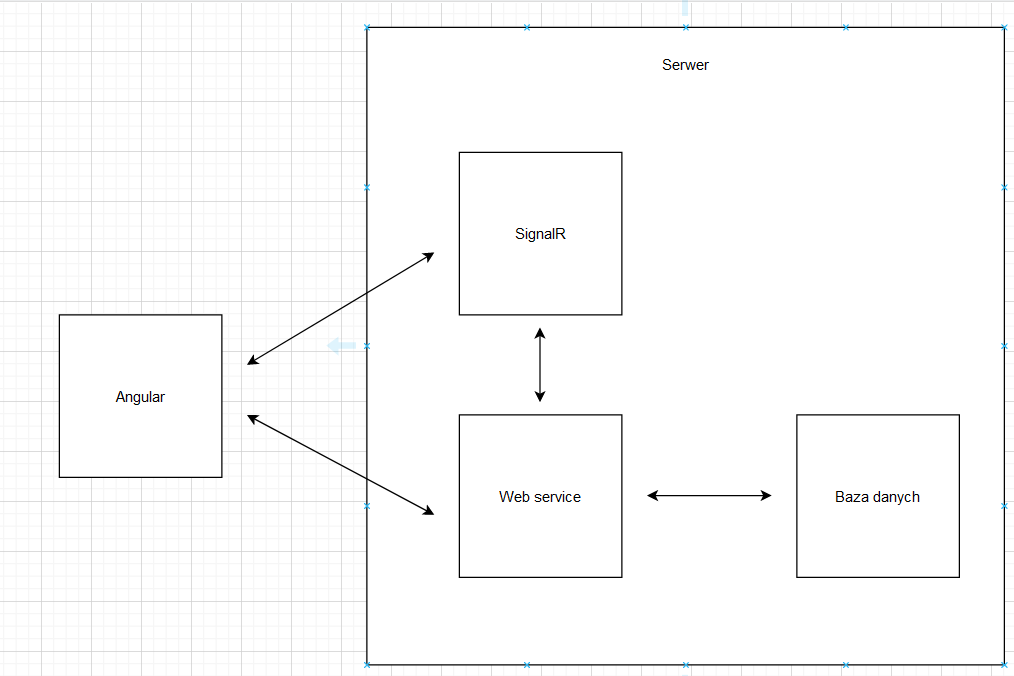
\includegraphics[width=0.7\linewidth]{diagramProjektu}
	\caption{}
	\label{fig:diagramprojektu}
\end{figure}
			
\subsection{Diagram Gantta}				%razem

\hspace*{0.7cm} Diagram Gantta dla naszego projektu przedstawia się następująco:

\begin{figure}[h]
	\centering
	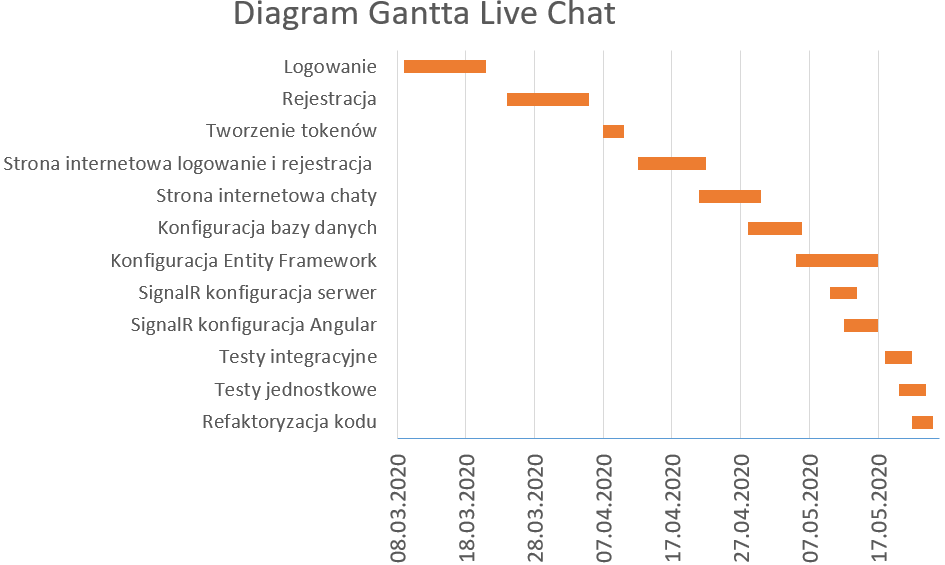
\includegraphics[width=0.8\linewidth]{diagramGantta}
	\caption{Diagram Gantta Live Chat}
	\label{fig:diagramgantta}
\end{figure}

\subsection{Use Cases}					%razem
Use case pokazują fukcjonalności projektu z podziałem na rodzaje użytkownik danej aplikacji. W live chat bedziemy wyrózniać dwa rodzaje użytkowników. Będzie to nowy user, który będzie miał możliwość jedynie rejestracji i drugi to będzie już utworzony user, który będzie mógł korzystać ze wszystkich korzyści programu.

\begin{figure}[h]
	\centering
	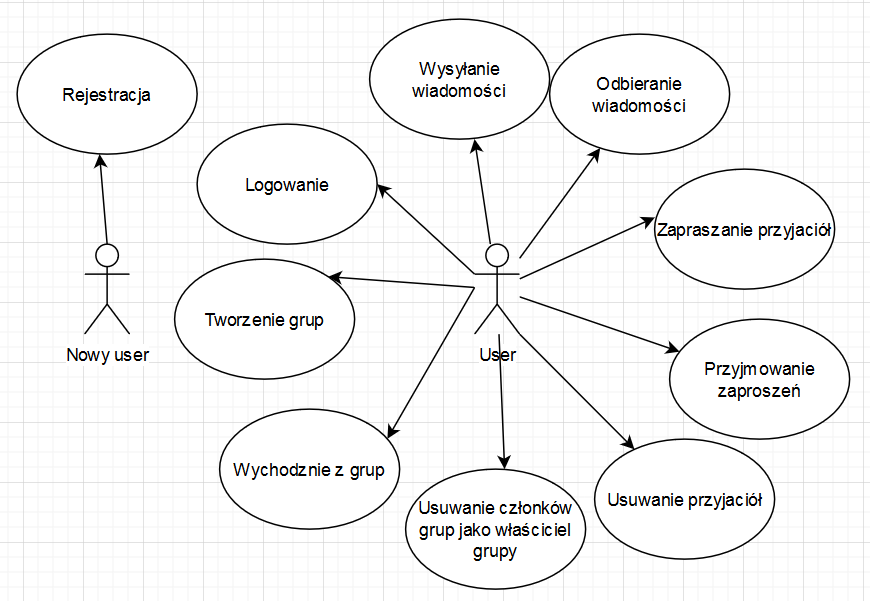
\includegraphics[width=0.7\linewidth]{usecase}
	\caption{}
	\label{fig:usecase}
\end{figure}

\subsection{Struktura bazy danych}  	%ja
Struktura bazy danych jest prosta i czytelna. Dla takiego projektu baza danych jest fundamentem. Musimy mieć miejsce do przechowywania informacji o użytkownikach, relacjach, wiadmościach czy czatach. Tabele opieraja się na relacjach między sobą. Sama struktura w mysql została wygenerowana przez Entity Framework Core, który zrobił w najbardziej optymalny i wydajny sposób.

\begin{figure}[ht!]
	\centering
	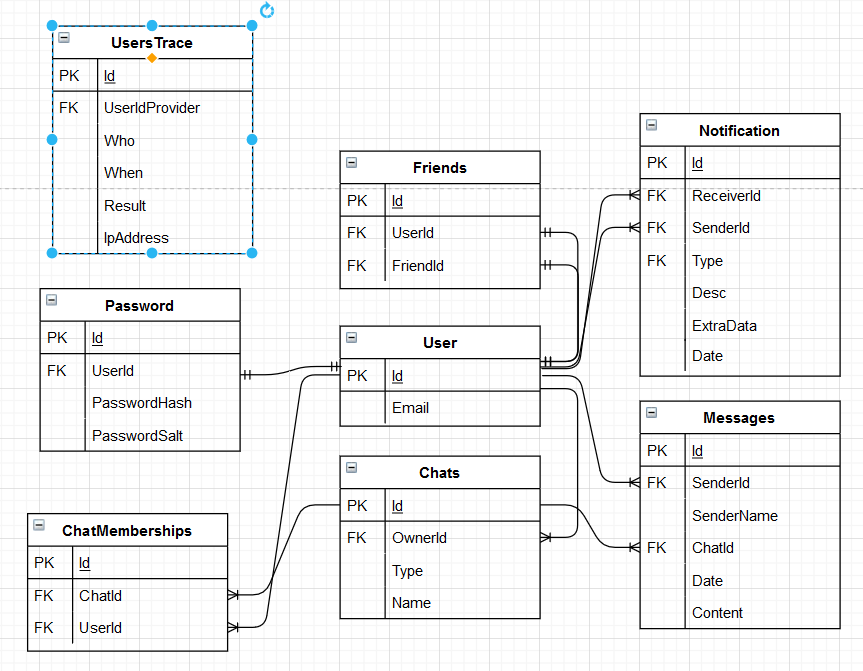
\includegraphics[width=0.7\linewidth]{diagrambazydanycj}
	\caption{}
	\label{fig:diagrambazydanycj}
\end{figure}


\subsection{Komunikacja z web serwisem} %kurek
Komunikacja z web serwisem została podzielona na część dla każdego usera i część tylko dla zalogowanych.
Po zalogowaniu wytwarzany jest token w User Controller i przesyłany z powrotem do klienta. Takowy token jest wykorzystywany do autoryzacji podczas dostępu do pozostałych kontrolerów. W przypadku SignalR, tylko zalogowani użytkownicy mogą się podłączyć. Wywoływana jest metoda RPC do walidacji użytkownika. Jest to druga część autoryzacji co czyni ją dwuetapową. Ta część polega na sprawdzeniu czy email zawarty w tokenie zgadza się z id usera. Wywoływana jest wówczas baza danych do pobrania emailu zawartego w rekodzie o danym id i przyrównanie tej wartości z wartością email zawartą w tokenie. Prosty diagram komunikacji z web serwisem jest następujący.

\begin{figure}[h]
	\centering
	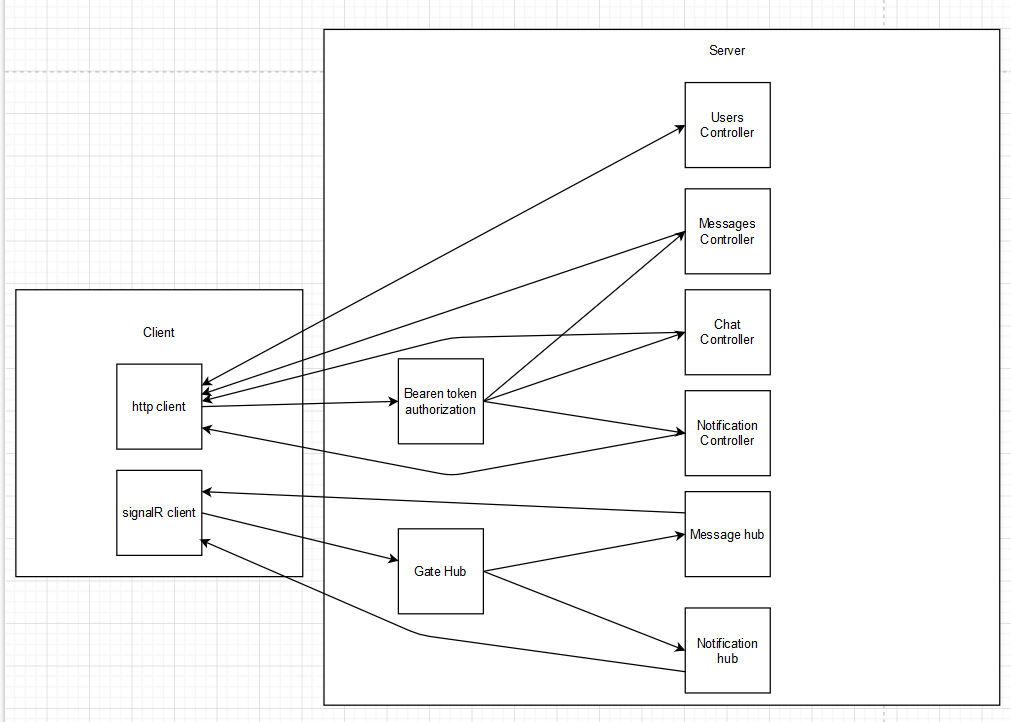
\includegraphics[width=0.7\linewidth]{komunikacjazwebserwisem}
	\caption{}
	\label{fig:komunikacjazwebserwisem}
\end{figure}


\subsection{Diagram klas}
Diagram klas przedstawia od strony czysto technicznej połączenia między poszczególnymi klasami, interfejsami czy typami prostymi. Pozwala zauważyć pewne założenia, schematy, które ułatwią implementowanie całego mechanizmu, aby uniknąć powtarzania się kodu czy zminimalizować ilość użytych linijek. 

\begin{figure}[ht!]
	\centering
	\includegraphics[width=1\linewidth]{C:/Users/ditri/Downloads/DiagramKlas(2)}
	\caption{}
	\label{fig:diagramklas2}
\end{figure}

\section{Implementacja}

\subsection{Modele bazy danych}				%ja - enity framework
\subsection{Modele DTO} 					%kurek
\subsection{Implementacja kontrolerów}		%razem
\subsection{Problemy i ich rozwiązania}		%razem

\section{Testy}

\subsection{Testy jednostkowe}   %ja
\subsection{Testy integracyjne}  %kurek

\section{Opis wkładu własnego w realizację projektu}

%ja
\subsection{Stworzenie i konfiguracja bazy danych}
\subsection{Stworzenie systemu logowania i rejestracji}
\subsection{Autoryzacja i autentykacja użytkowników}
\subsection{Konfiguracja środowiska i serwera}

%kurek
\subsection{Strona internetowa opracowana w Angular}
\subsection{Implementacja zarządzania wiadomościami}
\subsection{Implementacja zarządzania powiadomieniami}
\subsection{Implementacja zarządzania chatami}
\subsection{Obsługa SignalR}

\section{Podsumowanie}

\subsection{Wnioski}
\subsection{Do zrealizowania przy dalszym rozwoju}


\end{document}
